\documentclass[pdftex,a4paper,14pt,english,russian]{extarticle}

\usepackage[top=2cm,bottom=27mm,left=3cm,right=18mm]{geometry}
\usepackage[T2A]{fontenc}
\usepackage[utf8]{inputenc}
\usepackage[english,russian]{babel}
\usepackage[pdftex]{hyperref}
\usepackage{indentfirst}
\usepackage[pdftex]{graphicx}
\usepackage{amsmath}
\usepackage{amssymb}
\usepackage{ragged2e}
\usepackage{multirow}
\usepackage{algorithmic}
\usepackage[boxed]{algorithm}
\usepackage{tabularx}
\usepackage{listings}
\usepackage{xtab}
\usepackage{subfig}
\usepackage{hyphenat}
\usepackage{setspace}
\usepackage{fancyhdr}
\usepackage{float}

\pagestyle{fancyplain}
\fancyhf{}
\renewcommand{\headrulewidth}{0pt}
\rfoot{\fancyplain{}{\thepage}}

\linespread{1.2}
\floatname{algorithm}{Алгоритм}


\addto\captionsrussian{\renewcommand{\contentsname}{СОДЕРЖАНИЕ}}

% new commands
\newcommand\sign[1]{sign(#1)}

\begin{document}

%\begin{titlepage}
  \begin{center}
    \textsc{\small Министерство образования Республики Беларусь}\\[0.5cm]
    \textsc{\small Учреждение образования\\\large Белорусский государственный университет информатики и радиоэлектроники}\\[0.5cm]
    \begin{minipage}{\textwidth}
      \begin{flushleft}
        \begin{tabular}{ l l }
          Факультет & компьютерных систем и сетей\\
          Кафедра   & информатики
        \end{tabular}
      \end{flushleft}
    \end{minipage}\\[0.5cm]
    \begin{minipage}{\textwidth}
      \begin{flushright}
        \textit{К защите допустить:}\\
        Заведующий кафедрой информатики\\
        \underline{\hspace*{4.5cm}} Н.А. Волорова
      \end{flushright}
    \end{minipage}\\[1.5cm]
    \textsc{\large Пояснительная записка}\\
    \textsc{\small к дипломному проекту}\\
    \textsc{\small на тему}\\[0.5cm]
    \textbf{\large Программное обеспечение по управлению централизованными продажами в системе Bycard}\\[0.5cm]
    {\small БГУИР ДП \textbf{1-31 03 04 07 081} ПЗ}\\[0.5cm]
    {\small
      \begin{tabular}{ l l }
        Студент \hspace*{10cm} & О.О. Танасюк\\
        Руководитель & С.В. Актанорович\\
        Консультанты: &\\
        \hspace*{0.5cm}\emph{от кафедры информатики} & С.В. Актанорович\\
        \hspace*{0.5cm}\emph{по экономической части} & Т.Л. Слюсарь\\
        \hspace*{0.5cm}\emph{по охране труда} & А.А. Быков\\
        Нормоконтроллер & В.В. Шиманский\\
        &\\
        Рецензент &
      \end{tabular}
    }
    \vfill
    \textsc{\small Минск, 2014}
  \end{center}
\end{titlepage}

%\input{abstract.tex}
%\section*{Аннотация}
\thispagestyle{empty}

\begin{center}
  \begin{minipage}{0.8\textwidth}
    на дипломный проект ``Программное обеспечение по управлению централизованными продажами в системе Bycard'' студента УО ``Белорусский государственный университет информатики и радиоэлектроники'' Танасюка О.О.
  \end{minipage}
\end{center}

Дипломный проект выполнен на 6 листах формата А1 с пояснительной запиской на 61 странице (без приложений справочного или информационного характера). Пояснительная записка включает 6 глав, 18 рисунков, 22 литературных источников.

Темой дипломной работы является актуальная проблема компьютерного зрения --- захват людей на изображении и оценка их позы. Целью данного дипломного проекта является разработка приложения для захвата людей на изображении. ПО может быть внедрено в другие проекты с целью получения информации об объекте на изображении.

В первой главе дипломного проекта дается обзор оператора обнаружения краев Канни.

Во второй главе рассматривается метод усиления простых классификаторов, приводится алгоритм AdaBoost и его математическое обоснование.

Третья глава посвящена описанию дескриптора признаков Shape Context и изложению необходимого математического аппарата. Также излагаются возможные области применения.

В четвертой главе рассмотрены графические структуры, приведен метод захвата людей на изображении, совершен синтез изложенного в предыдущих разделах в единый фреймворк.

Пятая глава посвящена реализации пространственно\hyp{}антропометрической эргономической совместимости работника и технического средства при организации рабочего места.

В шестой главе приводится расчет себестоимости разработки, дается расчет экономического эффекта от использования программного средства. 

Глава ``Заключение'' содержит краткие выводы по дипломному проекту.

\newpage

%\input{feedback.tex}
%\input{review.tex}

%\setcounter{page}{5}
%\tableofcontents
%\newpage

%\section*{ВВЕДЕНИЕ}
\addcontentsline{toc}{section}{Введение}

В последние время, благодаря интенсивному развитию информационных технологий, в интернете можно купить практически все. Интернет-магазины уверенно держат свои позиции, ведь удобство такого шопинга оценили уже многие. Если ранее, чтобы приобрести билеты, необходимо было потратить достаточно много времени, сейчас данная задача значительно упрощена. Очереди и пробки на дорогах сменяются уютной атмосферой дома или офиса. Заказать необходимый билет можно в любое время суток и в любом месте.

Если вы задумываетесь о покупке билетов на мероприятия, будь то концерты, спектакли, сеансы в кинотеатре, семинары или выставки, вы наверняка и сами понимаете, что предпосылок отказаться от классической покупки, в пользу онлайн более чем достаточно. Проникновение Интернета в нашу жизнь становиться все более заметным. Объемы онлайн торговли растут с каждым днем, и мало кто захочет быть в стороне от этого процесса.

Преимущества, конечно же, очевидны, но все же стоит их перечислить:
\begin{itemize}
  \item Экономия времени. Для совершения онлайн покупки билетов через сайт продавца, нужно потратить 3-4 минуты. Что бы купить билет в кассе, надо потратить минимум 30 минут, обычно гораздо больше, особенно в крупных городах.
  \item Экономия денег. При покупке или бронировании билета традиционным способом, надо потратить деньги на транспорт или услуги курьера. Эта сумма, как правило, превышает размер комиссии сервисов.
  \item Возможность выбора мест. Пользователь сам выбирает понравившиеся места. 
  \item Возможность купить билеты заранее, и спланировать свое время рационально. 
\end{itemize}

Однако, всё ли так просто? Существует большое количество сервисов, которые предлагают довольно узкий спектр услуг, например, предложение купить билет в определённый кинотеатр или театр. Это, конечно, тоже весьма неплохо, но ориентироваться в огромном количестве онлайн-сервисов весьма непросто. Хотелось бы видеть систему, которая смогла бы предложить покупку билета на большой спектр мероприятий, будь то спектакль, концерт или выставка.

Но, опять же, с технической стороны к такой системе предъявляются серьёзные требования. Необходимо аггрегировать большое количество разноплановых подсистем, которые взаимодействуют с различными заведениями: кинотеатрами, театрами, концертными залами и др. 

Целью данного дипломного проекта являются описание и разработка программного обеспечения по управлению централизованными продажами через систему Bycard.

Была поставлена задача разработать такую систему, которая бы могла не только подключать заведения, но и позволила бы разрабатывать приложения для продажи билетов, для показа актуальной афиши с минимальными затратами. Это может быть любой клиент: сайт, мобильное приложение, информационный ресурс.

В данном дипломном проекте рассматривается процесс проектирования и реализации данной системы. Большое внимание уделяется контролю качества, созданию автоматической системы, которая контролирует корректность работы всех внешних и внутренних модулей, интегрированных в проект.

\newpage

%\section{Обзор предметной области}
В данном разделе будет произведён обзор предметной области задачи, решаемой в рамках дипломного проекта; рассмотрены вопросы о сущности
байесовых сетей и принципе их работы; приведена оценка сложности различных проблем, возникающих при применении вероятностных сетей для
решения прикладных задач. Также будут рассмотрены принципы работыалгоритмов вывода структуры по данным, реализованных
в программномобеспечении разработанном в рамках дипломного проекта, и произведеносравнение с существующим ПО для решения схожих задач.

\subsection{API как средство интеграции приложений}
API определяет функциональность, которую предоставляет программа (модуль, библиотека), при этом API позволяет абстрагироваться от того, как именно эта функциональность реализована.

Если программу (модуль, библиотеку) рассматривать как чёрный ящик, то API — это множество «ручек», которые доступны пользователю данного ящика, и которые он может вертеть и дёргать.

Программные компоненты взаимодействуют друг с другом посредством API. При этом обычно компоненты образуют иерархию — высокоуровневые компоненты используют API низкоуровневых компонентов, а те, в свою очередь, используют API ещё более низкоуровневых компонентов.

По такому принципу построены протоколы передачи данных по Интернет. Стандартный стек протоколов (сетевая модель OSI) содержит 7 уровней (от физического уровня передачи бит до уровня протоколов приложений, подобных протоколам HTTP и IMAP). Каждый уровень пользуется функциональностью предыдущего уровня передачи данных и, в свою очередь, предоставляет нужную функциональность следующему уровню.

Важно заметить, что понятие протокола близко по смыслу к понятию API. И то, и другое является абстракцией функциональности, только в первом случае речь идёт о передаче данных, а во втором — о взаимодействии приложений.
API библиотеки функций и классов включает в себя описание сигнатур и семантики функций.


\subsection{Проблемы, связанные с многообразием API}
Практически все операционные системы (UNIX, Windows, Mac OS и т. д.) имеют API, с помощью которого программисты могут создавать приложения для этой операционной системы. Главный API операционных систем — это множество системных вызовов.

В индустрии программного обеспечения общие стандартные API для стандартной функциональности имеют важную роль, так как они гарантируют, что все программы, использующие общий API, будут работать одинаково хорошо или, по крайней мере, типичным привычным образом. В случае API графических интерфейсов это означает, что программы будут иметь похожий пользовательский интерфейс, что облегчает процесс освоения новых программных продуктов.

С другой стороны, отличия в API различных операционных систем существенно затрудняют перенос приложений между платформами. Существуют различные методы обхода этой сложности — написание «промежуточных» API (API графических интерфейсов WxWidgets, Qt, GTK и т. п.), написание библиотек, которые отображают системные вызовы одной ОС в системные вызовы другой ОС (такие среды исполнения, как Wine, cygwin и т. п.), введение стандартов кодирования в языках программирования (например, стандартная библиотека языка C), написание интерпретируемых языков, реализуемых на разных платформах (sh, python, perl, php, tcl, Java и т. д.).

Также необходимо отметить, что в распоряжении программиста часто находится несколько различных API, позволяющих добиться одного и того же результата. При этом каждый API обычно реализован с использованием API программных компонент более низкого уровня абстракции.

Например: для того, чтобы увидеть в браузере строчку «Hello, world!», достаточно лишь создать HTML-документ с минимальным заголовком и простейшим телом, содержащим данную строку. Когда браузер откроет этот документ, программа-браузер передаст имя файла (или уже открытый дескриптор файла) библиотеке, обрабатывающей HTML-документы, та, в свою очередь, при помощи API операционной системы прочитает этот файл и разберётся в его устройстве, затем последовательно вызовет через API библиотеки стандартных графических примитивов операции типа «очистить окошко», «написать “Hello, world!” выбранным шрифтом». Во время выполнения этих операций библиотека графических примитивов обратится к библиотеке оконного интерфейса с соответствующими запросами, уже эта библиотека обратится к API операционной системы, чтобы записать данные в буфер видеокарты.

При этом практически на каждом из уровней реально существует несколько возможных альтернативных API. Например: мы могли бы писать исходный документ не на HTML, а на LaTeX, для отображения могли бы использовать любой браузер. Различные браузеры, вообще говоря, используют различные HTML-библиотеки, и, кроме того, всё это может быть (вообще говоря) собрано с использованием различных библиотек примитивов и на различных операционных системах.

Основными сложностями существующих многоуровневых систем API, таким образом, являются:
\begin{enumerate}
    \item сложность портирования программного кода с одной системы API на другую (например, при смене ОС);
    \item потеря функциональности при переходе с более низкого уровня на более высокий. Грубо говоря, каждый «слой» API создаётся для облегчения выполнения некоторого стандартного набора операций. Но при этом реально затрудняется, либо становится принципиально невозможным выполнение некоторых других операций, которые предоставляет более низкий уровень API.
\end{enumerate}



\subsection{Балансировка нагрузки}

Балансировка нагрузки  - миграции процессов или выбор компьютера для запуска нового процесса с целью равномерной загрузки всех компьютеров в вычислительной системе, оптимизации использования ресурсов и сокращения времени вычисления.

Балансировка нагрузки может быть использована для расширения возможностей компьютерной системы, состоящей более чем из одного сервера. Она также может позволить продолжать работу даже в условиях, когда несколько серверов вышли из строя. Благодаря этому растёт отказоустойчивость.

В системах с большим числом узлов часто возникают сбои, требующие вмешательства человека и временного отключения компьютера. Количество сбоев растёт пропорционально числу узлов. При этом необходимо, чтобы вычисления продолжались, так как зачастую расчётные программы не обладают встроенной возможностью сохранить своё состояние или из-за того, что результат нужно получить как можно быстрее. Здесь также возникает необходимость перенести работающий процесс на другой компьютер.

Аналогичная проблема возникает при совместном использовании группы компьютеров и в качестве кластера, и в качестве учебной аудитории. (Такое использование типично для учебных заведений.) Когда начинаются занятия, требуется освободить часть компьютеров для студентов и преподавателя, перенеся с них задачи на другие машины. При этом не всегда заранее известно, сколько машин понадобится.

Cистемы балансировки нагрузки применяются на серверных кластерах, межсетевых экранах, серверах инспектирования содержания (например, антивирусных и антиспамовых фильтрах) – всюду, где задача может быть разделена на параллельные слабо связанные задачи, требования которых к ресурсам могут переменными и даже труднопредсказуемыми. Под слабой связанностью подразумевается отсутствие необходимости частого обмена данными между процессами.

Система балансировки нагрузки должна постоянно отслеживать уровень нагрузки и состояние управляемых компьютеров с тем, чтобы на основании собранной информации в любой момент выбирать для  запуска или переноса очередного процесса  к тот сервер, на котором процесс сможет наилучшим образом работать.

\subsubsection{Балансировка нагрузки Web-серверов}

Cистема балансировки нагрузки Web-серверов - это инструментальное средство, выполненное в виде сетевого  устройства или программы и предназначенное для переадресации клиентских запросов на наименее загруженный или наиболее подходящий Web-сервер из группы машин, на которых хранятся зеркальные копии информационного ресурса [8]. Вся система представляются клиенту в виде некоего единого виртуального сервера. Возможность переноса запроса с одного сервера на другой не предусматривается.

\begin{figure}
  \centering
  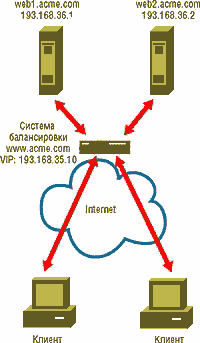
\includegraphics[width=0.3\textwidth]{images/balance-sys.png}
  \caption{Система балансировки нагрузки на 2 web-сервера}
\end{figure}

Для работы такой системы необходим алгоритм выбора сервера. Обычно в таких системах выбор происходит по принципу кругового списка, что эффективно в случае и одинаковых серверов и запросов, требующих одинаковое количество ресурсов.

\subsubsection{Избыточные системы балансировки}

Системы балансировки нагрузки - средства доступа к серверам Web, и потому выход такого средства из строя может повлечь за собой полное прекращение работы узла. Отсюда вывод: при планировании и реализации инфраструктуры с выравниванием нагрузок важно принимать во внимание отказоустойчивость средств балансировки, а также выбирать решения с широкой полосой пропускания, способные обеспечить высокую производительность системы в целом. В распоряжении администратора имеются две схемы организации избыточных систем балансировки нагрузки: первая предполагает, что одна система балансировки функционирует в активном режиме, а другая - находится в состоянии ожидания (active-and-standby type); вторая же схема предусматривает одновременное функционирование обеих систем балансировки (active-and-active type). Обе схемы предполагают наличие на одном узле двух экземпляров систем балансировки нагрузки.

При использовании метода одна система активна, а другая находится в состоянии ожидания, резервная система балансировки постоянно контролирует состояние главной системы, и, как только она  выходит из строя,  резервная система балансировки принимает на себя функции главной. Когда же главная система возобновляет работу, резервная передает ей управление трафиком и вновь переходит в режим ожидания.

В схеме с двумя активными системами балансировки нагрузки обе системы обслуживают трафик и подстраховывают друг друга. Представим для примера узел Web, состоящий из четырех серверов. Два из них обслуживаются первой системой балансировки нагрузки, и два - второй. Когда одна система балансировки выходит из строя, заботу обо всех четырех серверах берет на себя вторая система. Этот метод в полной мере использует ресурсы средств балансировки и повышает производительность узла.

\subsubsection{Больше, чем технология}

Компании, которые обслуживают информационные центры Web и занимаются электронной коммерцией, - далеко не единственные организации, применяющие системы балансировки нагрузки для управления трафиком и поддержания порядка в своих виртуальных хозяйствах. Многие компании взяли на вооружение средства балансировки для того, чтобы повысить производительность и доступность своих узлов Web.

Системы выравнивания нагрузки обеспечивают мониторинг нагрузок и состояния серверов, правильный выбор из пула серверов машины, способной наилучшим образом обработать запрос клиента, а также управление трафиком как внутри узла, так и в глобальном масштабе. Благодаря этому они становятся мощным оружием в конкурентной борьбе между компаниями, открывшими свои представительства в киберпространстве.

\subsection{Мониторинг состояния серверов}

\subsubsection{Внешний мониторинг}

При проведении внешнего мониторинга система балансировки нагрузки рассчитывает время отклика сервера, для чего направляет на сервер запрос и замеряет время ответа, например, по протоколу управления сообщениями Internet Control Message Protocol (ICMP).  Эти тесты позволяют системе проверить  готовность сервера к работе и узнать, сколько времени необходимо для передачи информации с сервера на систему балансировки и обратно. Если система балансировки нагрузки не получает отклика от сервера после нескольких последовательных запросов, считается, что данный сервер недоступен, работает с большой нагрузкой или произошёл какой-либо сбой.

Чтобы убедиться в правильности функционирования стека TCP сервера, система балансировки нагрузки предпринимает попытку установить соединение по протоколу TCP, для чего требуется осуществить состоящий из трех этапов обмен подтверждающими сообщениями. Сначала серверу направляется TCP-пакет, в котором значение бита SYN установлено равным 1. Если после этого система балансировки получает от сервера TCP-пакет, в котором значение бита SYN равно 1, а значение бита ACK тоже установлено равным 1, она направляет серверу второй TCP-пакет со значением бита SYN равным 0 и значением бита ACK равным 1. Если обмен подтверждающими сообщениями завершился успешно, значит, TCP-стек сервера функционирует нормально. Качество TCP-соединения с сервером оценивается системой как время, необходимое для выполнения всех трех этапов обмена подтверждающими сообщениями.

Лучшие средства балансировки нагрузки могут обеспечивать мониторинг времени отклика и готовности как самого Web-сервера, так и установленных на нем приложений еще одним способом: на сервер направляется запрос по протоколу HTTP на получение информационных материалов или адреса URL. Пусть именем начальной страницы сервера web1.kto-to.com будет index.html. Система балансировки нагрузки на рисунке 1.1 может инициировать предусмотренную по протоколу HTTP команду Get, запрашивая тем самым у сервера web1.kto-to.com содержимое страницы index.html. Если код возврата, направляемый системе Web-сервером, будет 200, значит, начальная страница на сервере web1.kto-to.com недоступна. Время отклика определяется системой балансировки нагрузки как время с момента отправки запроса на предоставление информации до момента получения кода возврата.

\subsubsection{Внутренний мониторинг}

Подробную информацию о таких существенных характеристиках сервера, как состояние центрального процессора, памяти, системной шины, шины ввода/вывода, сетевой интерфейсной платы, а также о ряде важных ресурсов системы и прикладных программ  может предоставить только внутренний мониторинг. Агенты, которые устанавливаются на каждом сервере, постоянно контролируют состояние своего компьютера и сообщают о нем системе балансировки. Внутренний мониторинг широко применяется в программных системах балансировки, но в аппаратных устройствах и в решениях на базе коммутаторов этот метод диагностики реализуется редко.

\subsection{Задача определения неисправности или отказа того или иного модуля системы}

В сложных распределённых системах одновременно выполняется множество операций, и в случае возникновения неисправности или отказа того или иного модуля системы бывает достаточно сложно сразу же определить причину неисправности или отказа. Поэтому важно наличие централизованного механизма получения и хранения сообщений и протоколов о работе программных модулей и подсистем в составе любого программного комплекса.

Каждый модуль системы, выполнив ту или иную операцию, должен добавить запись в соответствующий журнал операций. Использование журналов операций сокращает время на поиск причин возникающих неисправностей, так как становится возможным однозначно определить, после выполнения какой операции произошёл отказ.

Поскольку комплексы программ независимо от своей прикладной сферы должны иметь средства протоколирования операций, то целесообразно создать универсальный компонент для ведения журнала операций с возможностью подключать его к различным программам.

\newpage

%\section{ИСПОЛЬЗУЕМЫЕ ТЕХНОЛОГИИ}
\addcontentsline{toc}{section}{Используемые технологии}

Выбор технологий является важным предварительным этапом разработки сложных информационных систем. Платформа и язык программирования, на котором будет реализована система, заслуживает большого внимания, так как исследования показали, что выбор языка программирования влияет на производительность труда программистов и качество создаваемого ими кода. Ниже перечислены некоторые факторы, повлиявшие на выбор технологий:
\begin{itemize}
    \item разрабатываемое ПО должно работать на операционной системе Debian используемую в качестве серверной ОС;
    \item дальнейшей поддержкой проекта, возможно, будут заниматься разработчики, не принимавшие участие в выпуске первой версии;
    \item имеющийся разработчик имеет опыт работы с объекто-ориентированными и с функциональными языками программирования.
\end{itemize}

Основываясь на опыте работы имеющихся программистов разрабатывать ПО целесообразно на объектно-ориентированном языке PHP. Приняв во внимание необходимость обеспечения доступности дальнейшей поддержки ПО, возможно, другой командой программистов, целесообразно не использовать малоизвестные и сложные языки программирования.

\subsection{Язык программирования PHP}

PHP — скриптовый язык программирования общего назначения, интенсивно применяемый для разработки веб-приложений. В настоящее время поддерживается подавляющим большинством хостинг-провайдеров и является одним из лидеров среди языков программирования, применяющихся для создания динамических веб-сайтов.

Язык и его интерпретатор разрабатываются группой энтузиастов в рамках проекта с открытым кодом. Проект распространяется под собственной лицензией, несовместимой с GNU GPL.

В области программирования для сети Интернет, PHP — один из популярных сценарных языков (наряду с JSP, Perl и языками, используемыми в ASP.NET) благодаря своей простоте, скорости выполнения, богатой функциональности, кроссплатформенности и распространению исходных кодов на основе лицензии PHP.

Популярность в области построения веб-сайтов определяется наличием большого набора встроенных средств для разработки веб-приложений[8]. Основные из них:
\begin{itemize}
    \item автоматическое извлечение POST и GET-параметров, а также переменных окружения веб-сервера в предопределённые массивы;
    \item взаимодействие с большим количеством различных систем управления базами данных (MySQL, MySQLi, SQLite, PostgreSQL, Oracle (OCI8), Oracle, Microsoft SQL Server, Sybase, ODBC, mSQL, IBM DB2, Cloudscape и Apache Derby, Informix, Ovrimos SQL, Lotus Notes, DB++, DBM, dBase, DBX, FrontBase, FilePro, Ingres II, SESAM, Firebird / InterBase, Paradox File Access, MaxDB, Интерфейс PDO);
    \item автоматизированная отправка HTTP-заголовков;
    \item работа с HTTP-авторизацией;
    \item работа с cookies и сессиями;
    \item работа с локальными и удалёнными файлами, сокетами;
    \item обработка файлов, загружаемых на сервер;
    \item работа с XForms.
\end{itemize}

В настоящее время PHP используется сотнями тысяч разработчиков. Согласно рейтингу корпорации TIOBE, базирующемся на данных поисковых систем, в июне 2013 года PHP находился на 5 месте среди языков программирования. К крупнейшим сайтам, использующим PHP, относятся Facebook, Wikipedia и др.


\subsection{Фреймворк Symfony}


Symfony — свободный каркас, написанный на PHP5, который использует паттерн Model-View-Controller.

Symfony предлагает быструю разработку и управление веб-приложениями, позволяет легко решать рутинные задачи веб-программиста. Работает только с PHP 5 (>=5.2.4 и желательно не 5.2.9 для Symfony 1.4, >=5.3.2 для Symfony 2). Имеет поддержку множества баз данных (MySQL, PostgreSQL, SQLite или любая другая PDO-совместимая СУБД). Информация о реляционной базе данных в проекте должна быть связана с объектной моделью. Это можно сделать при помощи ORM инструмента. Symfony поставляется с двумя из них: Propel и Doctrine.

Symfony бесплатен и публикуется под лицензией MIT. Проект спонсируется французской компанией Sensio.

\subsection{Паттерн  Model-View-Controller}

Model-view-controller (MVC, «модель-представление-поведение», «модель-представление-контроллер», «модель-вид-контроллер») — схема использования нескольких шаблонов проектирования, с помощью которых модель данных приложения, пользовательский интерфейс и взаимодействие с пользователем разделены на три отдельных компонента таким образом, чтобы модификация одного из компонентов оказывала минимальное воздействие на остальные. Данная схема проектирования часто используется для построения архитектурного каркаса, когда переходят от теории к реализации в конкретной предметной области.

Основная цель применения этой концепции состоит в разделении бизнес-логики (модели) от её визуализации (представления, вида). За счет такого разделения повышается возможность повторного использования. Наиболее полезно применение данной концепции в тех случаях, когда пользователь должен видеть те же самые данные одновременно в различных контекстах и/или с различных точек зрения. В частности, выполняются следующие задачи:
\begin{enumerate}
    \item к одной модели можно присоединить несколько видов, при этом не затрагивая реализацию модели. Например, некоторые данные могут быть одновременно представлены в виде электронной таблицы, гистограммы и круговой диаграммы;
    \item не затрагивая реализацию видов, можно изменить реакции на действия пользователя (нажатие мышью на кнопке, ввод данных), для этого достаточно использовать другой контроллер;
    \item ряд разработчиков специализируется только в одной из областей: либо разрабатывают графический интерфейс, либо разрабатывают бизнес-логику. Поэтому возможно добиться того, что программисты, занимающиеся разработкой бизнес-логики (модели), вообще не будут осведомлены о том, какое представление будет использоваться;
\end{enumerate}

Концепция MVC позволяет разделить данные, представление и обработку действий пользователя на три отдельных компонента:
\begin{itemize}
    \item модель (англ. Model). Модель предоставляет знания: данные и методы работы с этими данными, реагирует на запросы, изменяя своё состояние. Не содержит информации, как эти знания можно визуализировать.
    \item представление, вид (англ. View). Отвечает за отображение информации (визуализацию). Часто в качестве представления выступает форма (окно) с графическими элементами.
    \item контроллер (англ. Controller). Обеспечивает связь между пользователем и системой: контролирует ввод данных пользователем и использует модель и представление для реализации необходимой реакции.
\end{itemize}

Важно отметить, что как представление, так и контроллер зависят от модели. Однако модель не зависит ни от представления, ни от контроллера. Тем самым достигается назначение такого разделения: оно позволяет строить модель независимо от визуального представления, а также создавать несколько различных представлений для одной модели.

Для реализации схемы Model-View-Controller используется достаточно большое число шаблонов проектирования (в зависимости от сложности архитектурного решения), основные из которых «наблюдатель», «стратегия», «компоновщик».

Наиболее типичная реализация отделяет вид от модели путем установления между ними протокола взаимодействия, используя аппарат событий (подписка/оповещение). При каждом изменении внутренних данных в модели она оповещает все зависящие от неё представления, и представление обновляется. Для этого используется шаблон «наблюдатель». При обработке реакции пользователя вид выбирает, в зависимости от нужной реакции, нужный контроллер, который обеспечит ту или иную связь с моделью. Для этого используется шаблон «стратегия», или вместо этого может быть модификация с использованием шаблона «команда». А для возможности однотипного обращения с подобъектами сложно-составного иерархического вида может использоваться шаблон «компоновщик». Кроме того, могут использоваться и другие шаблоны проектирования, например, «фабричный метод», который позволит задать по умолчанию тип контроллера для соответствующего вида.

\subsection{Реляционная СУБД MySQL}

MySQL — свободная реляционная система управления базами данных. Разработку и поддержку MySQL осуществляет корпорация Oracle, получившая права на торговую марку вместе с поглощённой Sun Microsystems, которая ранее приобрела шведскую компанию MySQL AB. Продукт распространяется как под GNU General Public License, так и под собственной коммерческой лицензией. Помимо этого, разработчики создают функциональность по заказу лицензионных пользователей. Именно благодаря такому заказу почти в самых ранних версиях появился механизм репликации.MySQL является решением для малых и средних приложений. Входит в состав серверов WAMP, AppServ, LAMP и в портативные сборки серверов Денвер, XAMPP. Обычно MySQL используется в качестве сервера, к которому обращаются локальные или удалённые клиенты, однако в дистрибутив входит библиотека внутреннего сервера, позволяющая включать MySQL в автономные программы.

Гибкость СУБД MySQL обеспечивается поддержкой большого количества типов таблиц: пользователи могут выбрать как таблицы типа MyISAM, поддерживающие полнотекстовый поиск, так и таблицы InnoDB, поддерживающие транзакции на уровне отдельных записей. Более того, СУБД MySQL поставляется со специальным типом таблиц EXAMPLE, демонстрирующим принципы создания новых типов таблиц. Благодаря открытой архитектуре и GPL-лицензированию, в СУБД MySQL постоянно появляются новые типы таблиц.

\newpage

\section{ПРОЕКТИРОВАНИЕ ПРОГРАММНОГО КОМПЛЕКСА}
\addcontentsline{toc}{section}{Проектирование программного комплекса}

Важным этапом разработки любого программного комплекса является его проектирование. Любой проект, связанный с созданием программного продукта, требует предварительного проектирования, построения структуры и планирования сроков разработки. После предварительного утверждения плана разработки и выбора используемых технологий и структуры программного продукта начинается его реализация.

В данном разеделе будет произведен анализ основных требований; рассмотрены этапы проектирования основных модулей системы.

\subsection{Анализ требований и постановка задачи}

Разработанный программный прогаммный комплекс по управлению централизованными продажами в системе Bycard должен предоставить единый интерфейс для покупки билетов на мероприятия. Это значительно облегчит разработку клиентов для продажи билетов: мобильных приложений, сайта.

Система должна аггрегировать актуальную информацию о проходящих мероприятиях: расписание, цены на билеты, наличие доступных для продажи мест, возможность покупки билета онлайн. А также предоставить информационными ресурсам удобный механизм интерграции, благодаря которому будет возможность размещать актуальную афишу мероприятий на сторонних сайтах, показывать кнопки для покупки билета.

Большое значение имеют затраты на подключение к системе группы новых объектов, синхронизации данных между ними. Необходимо разработать механизм, который позволит подключать к системе объекты для продажи билетов с минимальными затратами.

\subsection{API}

Один из главных модулей системы. В данном разделе приводится его описание. Затронуты вопросы о стабильности и надежности работы всей системы в целом. Описаны механизмы, которые позволяют балансировать нагрузку на внешних подсистемах.

\subsubsection{Структура}

Данный модуль системы предоставляет общий интерфейс для общения с объектами, подключёнными к системе. Объекты могут иметь различные интерфейсы обмена данными. Например, система для продажи билетов, установленная в кинотеатре наверняка отличается от той, что установлена в театрах, филармонии, концертных залах и т.д. Поэтому логично будет написать для каждой группы объектов отдельный клиент, который будет необходимый интерфейс методов. Для кинотеатров это будет одна реализация, для театров - другая. Обобщённая структура изображена на рисунке ~\ref{fig:api-struct}:

\begin{figure}[H]
  	\centering
 	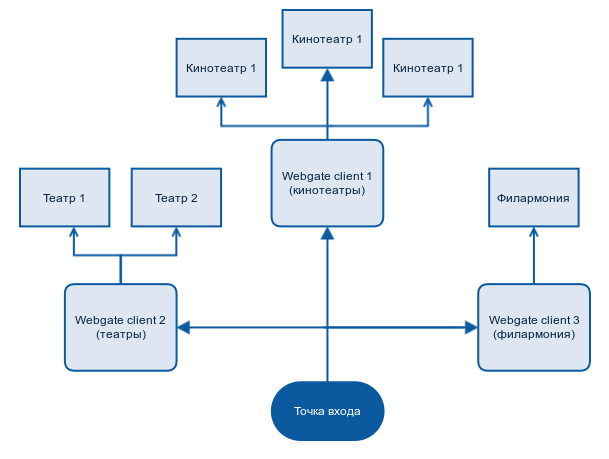
\includegraphics[width=1\textwidth]{images/api-struct.png}
  	\caption{Структура API}
    \label{fig:api-struct}
\end{figure}


В терминах проекта будем далее называть объект, подключенный к системе вебгейтом, а клиент для работы с ним - вебгейт-клиентом. Каждый клиент для вебгейта должен реализовывать необходимый минимум методов, определенных в интерфейсе WebgateClientInterface. Это методы для для реализации фукнции покупки билета: метод блокировки и разблокировки места, создания и отмены заказа. Метод getOrder используется в чекере, который будет описан дальше. Метод getPerformances нужен для получения списка мероприятий, цен на события, которые проходят в конкретном объекте. Система с заданной периодичностью получает актуальную информацию, обновляет её и сохраняет для дальнейшего использования. Приведем список основных методов интерфейса:


\begin{itemize}
    \item getPerformances();
	\item authorize();
	\item lockPlace();
	\item unlockPlace();
	\item createOrder();
	\item cancelOrder();
	\item unlockPlaces();
	\item getPlaces();
	\item addPayment();
	\item returnPlace();
	\item getOrder();
\end{itemize}


\subsubsection{Обработка запроса}

Одна из основных задач системы снизить нагрузку на конечные вебгейты. Для этого разработан механизм отложенных запросов. Согласно этому механизму некоторые запросы не обязательно выполять сразу. В данном случае запрос помещается в очередь отложенных запросов. Запросы из очереди выполняются с задержкой, в зависимости от загруженности конечно вебгейта. Данный механизм позволяет значительно снизить загруженность сервера на объекте. Алгоритм обработки запроса к апи приведен на рисунке ~\ref{fig:request-timeline}:

\begin{figure}[H]
  	\centering
 	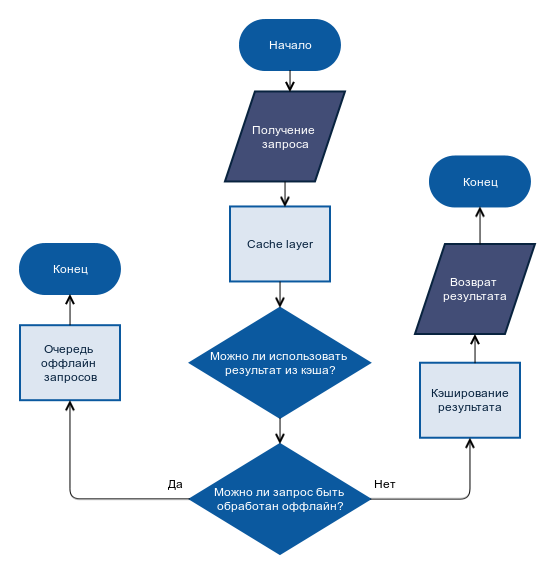
\includegraphics[width=1\textwidth]{images/request-timeline.png}
  	\caption{Алгоритм обработки запроса к API}
    \label{fig:request-timeline}
\end{figure}

Обработчик очереди запросов работает отдельно для каждого из вебгейта. На очередной итерации выбирается еще не выполненный запрос и делается попытка его выполнить. Если запрос выполнен, успешно и вернулся корректный ответ по нему, то он помечается как выполненный. Выполненные запросы в дальнейшем никак не обрабатывается. Однако возможен вариант, при котором запрос выполнился некорекктно, либо мы система не получила корректного ответа по нему, и не известно, отработал он на вебгейта или нет. В данном случае запрос будет обработан повторно через некоторое время либо снят из очереди по истечении количества попыток или потере актуальности. Данный механизм возможен и для онлайн-запросов, который сразу не попадают в очередь отложенных. Если онлайн-запрос не отработал корректно, но его выполнение критично - он может быть помещен в очередь отложенных запросов. После этого его обработка будет проходить по схеме, изложенной выше.

Важным дополнением к задаче является кэширующий слой. Большинство запросов, связанных с получением данных, можно кэшировать на определенный период. В данном случае запрос на конечный вебгейт не посылается вовсе, а данные берутся из кэша системы. Отметим одно из самых частых обращений к апи - запрос на получение карты. Его можно кэшировать на небольшой промежуток времени.


\subsubsection{Интеграция с информационными ресурсами}

Одной из задач системы является аггрегирование актуальной афиши мероприятий. Это даёт возможность делиться данной информацией с различными информационными ресурсами. Многие ресурсы размещают у себя афишу кино, театров и других развлекательных мероприятий. Упрощённая схема взаимодействия показана на рисунке ~\ref{fig:ir-schema}.

\begin{figure}
  	\centering
 	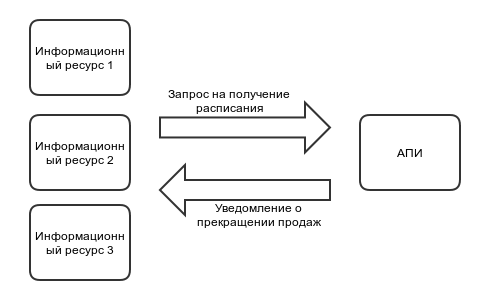
\includegraphics[width=1\textwidth]{images/ir-schema.png}
  	\caption{Упрощенная схема взаимодействия с информационными ресурсами}
    \label{fig:ir-schema}
\end{figure}

API предоставляет возможность выгрузить расписание полностью. С другой стороны хорошо иметь возможность не выгружать всё полностью каждый раз, а получать только обновления. Для этого реализован метод, который позволяет получить все обновления после определенного времени, которое задаст информационный ресурс.

Также есть возможность посылать уведомления со стороны системы о каких-либо изменениях. Например о том, что все билеты на какой-либо сеанс проданы. Информационный ресурс при желании может их тоже обрабатывать.

\subsection{Мониторинг работоспособности}

Через систему каждый день проходит большое количество операций по покупке билетов. Для большой системы, в которой есть большое количество независимых подсистем, необходим механизм который бы автоматически проверял работоспособность и корректную работу подсистем и, в случае найденной неисправности, пытался в автоматическом режиме исправить проблему, либо, при невозможности автоматического восстановления работы, посылал сигнал оператору, который пытается уже решить проблему в ручном режиме.

Мониторинг рабоспособности билетных операций - одна из важных задач. На рисунке ~\ref{fig:checker.png} изображен алгоритм работы чекера заказов. Рассмотрим его в качестве примера

Выбирается очередной, еще не проверенный заказ. Для каждого билета в заказе делается проверка на то, что данный билет существует в базе конечного вебгейта, который чаще всего расположен в месте проведения мероприятия. Проверяется соотвествие мест, цена, дата и время сеанса. Если информация совпадает - алгоритм заканчивает работу над текущим заказом и переходит к следующему. Иначе делается попытка исправить данные в вебгейте в автоматическом режим, чтобы информация на билете совпадала с информацией из вебгейта. Если в итоге не получается решить проблему, заказ помечается соответсвующей меткой, и переходит к оператору. При любом варианте далее заказ отправляется на повторную проверку до момента, пока чекер не скажет, что он полностью корректный.

\begin{figure}
  	\centering
 	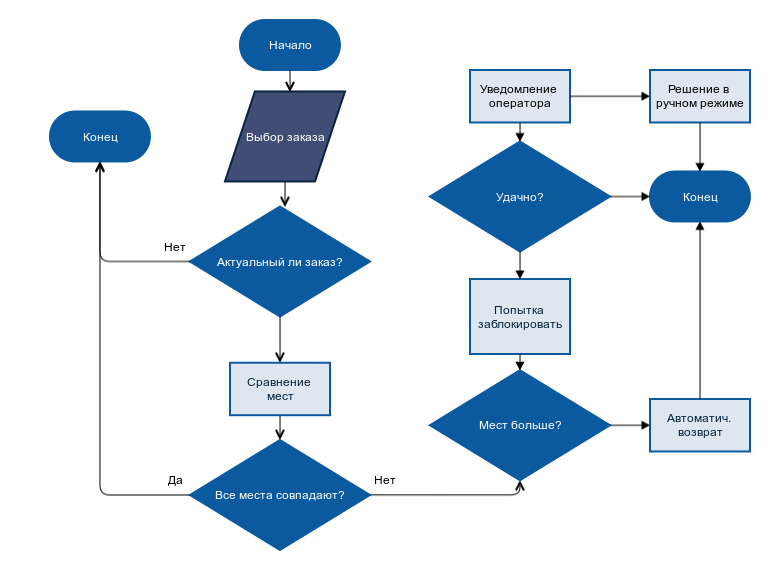
\includegraphics[width=1\textwidth]{images/checker.png}
  	\caption{Алгоритм работы чекера}
    \label{fig:checker.png}
\end{figure}


Таким образом обеспечивается корректность работы билетных операций, уменьшается риск возникновения непредвиденных ситуаций. Так как операции преимущественно выполняется в автоматическом режиме, уменьшается риск человеческой ошибки. 


Кроме чекера заказов в билетных операциях в системе есть чекеры работоспособности вебгейтов и других подсистем, таких как инфокиоски для доставки билетов и т.д.
Постоянный мониторинг в автоматическом режиме способствуют надёжной работе всей системы в целом.


\subsection{Панель мониторинга оператора}


Панель мониторинга и соответствующие ей веб-части содержат большое количество полезных данных о ходе продаж, статистике и качестве работы всех подсистем. Поскольку панель  постоянно подключена к источникам данных, сведения в ней своевременно обновляются и, как правило, являются интерактивными.

Панель мониторинга оператора предназначена для просмотра статистики, мониторинга работоспособности подсистем в ручном режиме. Как уже было отмечено, в ней отображаются  задачи которые не удалось решить автоматической системе. Схема того, как оператор взаимодействует с автоматической системой представлена на рисунке ~\ref{fig:panel.png}.

\begin{figure}[H]
    \centering
  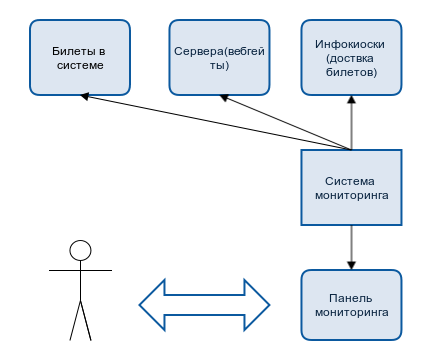
\includegraphics[width=1\textwidth]{images/panel.png}
    \caption{Панель мониторинга оператора}
    \label{fig:panel.png}
\end{figure}

Также панель мониторинга поддерживают следующие возможности:

\begin{itemize}
  \item изменение уровня детализации данных;
    \item поиск нужных данных путем фильтрации;
    \item изучение данных с помощью действий в различных меню;
    \item формирование отчетов;
    \item экспорт отчетов;
  \item просмотр статистики.
\end{itemize}


Здесь могут быть представлены отчеты самых разных типов, каждый из которых выполняет определенную задачу. Некоторые отчеты формируются из сведений о продажах на стороне API, другие - из сведений на стороне платежных систем, третьи - из сведений на стороне вебгейтов. Также существует механизм сверки отчетности, который при правильной настройке сообщает о проблемах, связанных с различиями в отчетах.
















\newpage
%\section{Обеспечение электробезопасности при эксплуатации проектируемого устройства}

Первоначальные стадии разработки дипломного проекта выполнялись на предприятии «Информационные системы Байкард» во время прохождения преддипломной практики. Для использования системы необходимо произвести настройку серверов, терминалов для доставки билетов. Таким образом, нужно иметь дело с электрооборудованием. В настоящем разделе рассматриваются вопросы, связанные с обеспечением электробезопасности на предприятии.

В качестве примера рассмотрим терминал для доставки билетов. Схема электропитания терминала изображена на рисунке ~\ref{ot-el-schema}

\begin{figure}
  	\label{ot-el-schema}
  	\centering
  	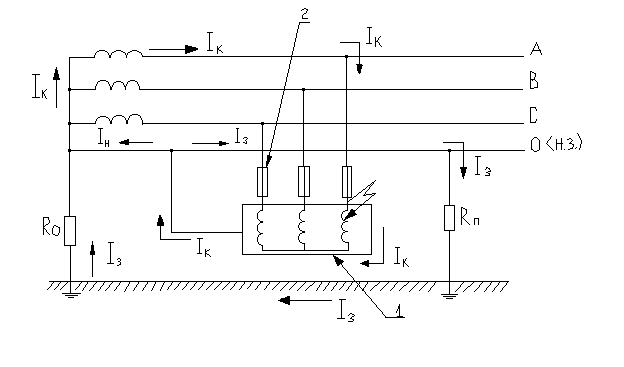
\includegraphics[width=1\textwidth]{images/ot-el-schema.png}
  	\caption{Схема электропитания}
\end{figure}

Внутренние устройства монтируются в корпус, у которого есть подключение к стандартной сети 220 В. Основные свойства блока питания YP-350J-AA:

\begin{itemize}
    \item универсальный вход 100…264 В переменного тока; 
    \item выходная мощность: 350 Вт; 
    \item не боится провалов входного напряжения; 
    \item встроенный корректор коэффициента мощности; 
    \item коэффициент мощности >0,95; 
    \item комплекс защит: от перегрузки и перенапряжения.
\end{itemize}

Поражение электрическим током возможно как при случайном прикосновении его  непосредственно к токоведущим частям, так и к неметаллическим нетоковедущим элементам электрооборудования (к корпусу электрических машин, трансформаторов, светильников и т.п.), которые могут оказаться под напряжением в результате какой – либо аварийной ситуации (замыкания фазы на корпус, повреждение изоляции и т.п.).

Оценка опасности электропоражения заключается в сравнении максимально возможных токов электропоражения, полученных с помощью измерения или расчёта, с предельно допустимыми их значениями. Предельно допустимые напряжения прикосновения \( \text{U}_{\text{пр}} \) и токи, проходящие через человека \( \text{I}_{\text{h пд}} \) при нормальном (неаварийном) режиме работы электроустановки приведены в таблице ~\ref{ot-tab}:

\begin{table}[h]
\label{ot-tab}
\center
\begin{xtabular}{|l|l|l|ll}
	\cline{1-3}
	\multirow{2}{*}{Род и частота тока} & \multicolumn{2}{l|}{Предельно допустимые значения} &  &  \\ \cline{2-3}
	& \multicolumn{1}{|>{}p{0.20\textwidth}|} {Uпр}                      & \multicolumn{1}{|>{}p{0.20\textwidth}|} {Ih}                      &  &  \\ \cline{1-3}
	\multicolumn{1}{|>{}p{0.33\textwidth}|}{Переменный, 50Гц} & 2 & 0,3 &  &  \\ \cline{1-3}
	\multicolumn{1}{|>{}p{0.33\textwidth}|}{Постоянный} & 8 & 1,0 &  &  \\ \cline{1-3}
\end{xtabular}
\end{table}

Оценка опасности позволяет определить необходимость применения способов и средств защиты, а возможные или фактические и предельно допустимые значения тока, проходящего через тело человека, и напряжения прикосновения служат исходными данными для их выбора, проектирования и расчёта.

Защитное зануление и заземление являются наиболее распространенными, весьма эффективными и простыми мерами защиты от поражения электрическим током при появлении напряжения на металлических нетоковедущих частях (металлических корпусах оборудования).

Опасность поражения электрическим током при прикосновении к корпусу и другим нетоковедущим частям электрооборудования, оказавшимся под напряжением, может быть устранена быстрым отключением поврежденного электрооборудования от питающей сети. Для этой цели используется зануление, принципиальная схема которого в сети трехфазного тока показана на рисунке 2:

\begin{figure}
  	\label{ot-zanul}
  	\centering
  	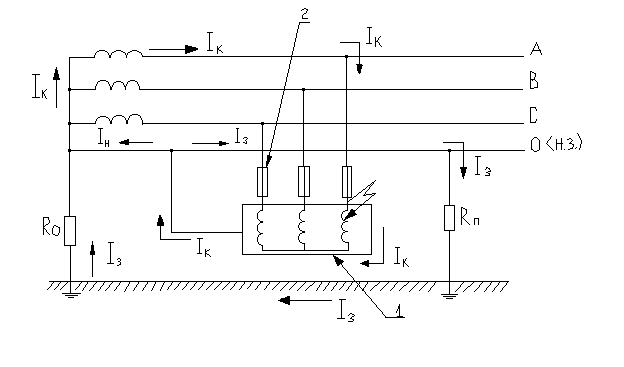
\includegraphics[width=1\textwidth]{images/ot-zanul.png}
  	\caption{Принципиальная схема зануления}
\end{figure}

Обозначения на схеме (рисунок 2):

1 --- корпус;

2 --- аппараты защиты от токов короткого замыкания (предохранители, автоматические выключатели.);

\( \text{R}_{\text{0}} \) --- сопротивление заземления нейтрали источника тока;

\( \text{R}_{\text{п}} \) --- сопротивление повторного заземления нулевого защитного проводника;

\( \text{I}_{\text{к}} \) --- ток короткого замыкания;

\( \text{I}_{\text{н}} \) --- часть тока короткого замыкания, протекающая через нулевой проводник;

\( \text{I}_{\text{з}} \) --- часть тока короткого замыкания, протекающая через землю;

0 (н.з.) --- нулевой защитный проводник.

Зануление – это преднамеренное электрическое соединение с нулевым защитным проводником металлических нетоковедущих частей, которые могут оказаться под напряжением.
Принцип действия зануления – превращение замыкания на корпус в однофазное короткое замыкание (между фазным и нулевым проводником) с целью вызвать большой ток, способный обеспечить срабатывание защиты и автоматически отключить поврежденное электрооборудование от питающей сети. В качестве отключающих аппаратов используются: плавкие предохранители, автоматические выключатели, магнитные пускатели и т.д. При этом необходимо учесть, что с момента возникновения аварии (замыкания на корпус) и до момента автоматического отключения поврежденного оборудования от сети имеется небольшой промежуток времени, в течение которого прикосновение к корпусу опасно, так как корпус находится под напряжением Uф  (рисунок 2)  и отключение его от сети еще не произошло. В этот период сказывается защитная функция заземления корпуса оборудования через нулевой защитный проводник.

Принцип действия зануления – превращение замыкания на корпус в однофазное короткое замыкание (между фазным и нулевым проводником) с целью вызвать большой ток, способный обеспечить срабатывание защиты и автоматически отключить поврежденное электрооборудование от питающей сети. В качестве отключающих аппаратов используются: плавкие предохранители, автоматические выключатели, магнитные пускатели и т.д. При этом необходимо учесть, что с момента возникновения аварии (замыкания на корпус) и до момента автоматического отключения поврежденного оборудования от сети имеется небольшой промежуток времени, в течение которого прикосновение к корпусу опасно, так как корпус находится под напряжением Uф  (рисунок 2)  и отключение его от сети еще не произошло. В этот период сказывается защитная функция заземления корпуса оборудования через нулевой защитный проводник.

Отключение поврежденной установки от питающей сети произойдет, если значение тока однофазного короткого замыкания, которое искусственно создается в цепи, будет больше (или равно) значения тока срабатывания автоматического выключателя (или номинального тока плавкой вставки предохранителя) и выполняется следующее условие:

где k --- коэффициент кратности тока, выбирается в зависимости от типа защиты электроустановки.

Для расчета зануления используем рисунок 3.

\begin{figure}
  	\label{ot-zanul}
  	\centering
  	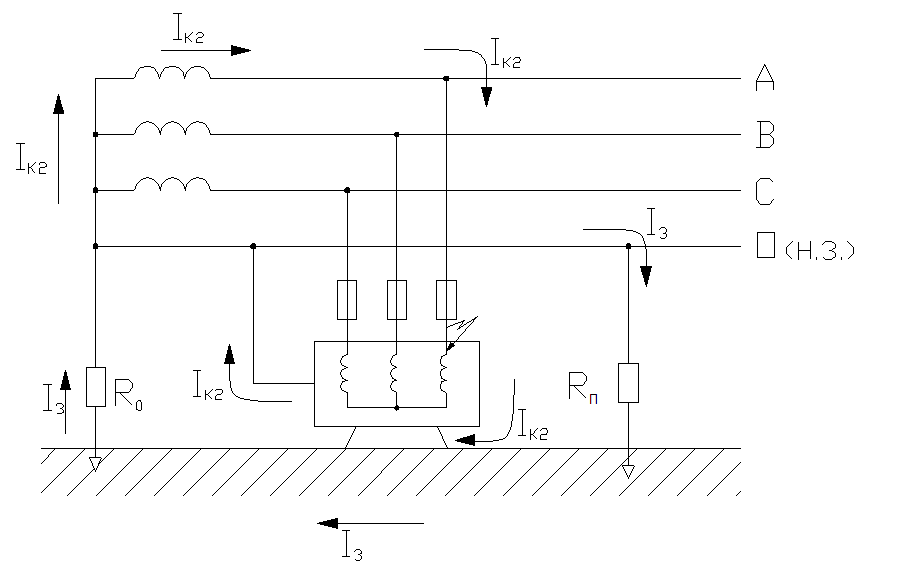
\includegraphics[width=1\textwidth]{images/ot-zanul2.png}
  	\caption{Зануление}
\end{figure}

Расчет зануления сводится к проверке соблюдения следующего условия:

\begin{displaymath}
  \text{I}_{\text{К2}} >= \text{I}_{\text{К1}}
\end{displaymath}

Для этого необходимо определить:

\begin{enumerate}
	\item наименьшее допустимое значение тока (\(\text{I}_{\text{К1}}\)) короткого замыкания, при котором произойдет срабатывание защиты и поврежденное оборудование отключится от сети;
	\item действительное значение тока однофазного короткого замыкания, которое будет иметь место в схеме при возникновении аварии (\(\text{I}_{\text{К2}}\)).
\end{enumerate}

Определяем величину тока:

\begin{displaymath}
  \text{I}_{\text{К1}} = k\cdot\text{I}_\text{ном},
\end{displaymath}

где \(\text{I}_\text{ном}\) --- номинальный ток плавкой вставки предохранителя электродвигателя, \(\text{I}_\text{ном}\) = 10А;

k --- коэффициент кратности, k = 1,25.

\begin{displaymath}
  \text{I}_{\text{К1}} = 1,25\cdot10 = 12,5\text{ (А)}
\end{displaymath}

Определяем полное сопротивление петли “фаза–нуль”:

\begin{displaymath}
  \text{Z}_\text{П} = \sqrt{(\text{R}_\text{ф}+\text{R}_\text{нз})^2+(\text{Х}_\text{ф}+\text{Х}_\text{нз}+\text{Х}_\text{п})^2},
\end{displaymath}

где \(\text{Р}_\text{ф}\), \(\text{Р}_\text{нз}\) --- активные сопротивления фазного и нулевого защитного проводников, \(\text{Р}_\text{ф}\) = 0,09 Ом, \(\text{Р}_\text{нз}\) = 0,308 Ом;

\(\text{Х}_\text{ф}\), \(\text{Х}_\text{нз}\) --- внутренние индуктивные сопротивления фазного и нулевого защитного проводников, \(\text{Х}_\text{ф}\) = 0,033 Ом, \(\text{Х}_\text{нз}\) = 0,308 Ом;

\(\text{Х}_\text{п}\) --- внешнее индуктивное сопротивление петли “фаза–нуль” (0,02 Ом).

\begin{displaymath}
  \text{Z}_\text{П} = \sqrt{(0,9+0,308)^2+(0,033+0,308+0,02)^2} = 1,21 \text{ (Ом)}.
\end{displaymath}

Находим действительное значение тока однофазного короткого замыкания, проходящего в схеме в аварийном режиме:

\begin{displaymath}
  \text{I}_\text{К2} = \frac{\text{U}_\text{Ф}}{\frac{\text{Z}_\text{T}}{3}+\text{Z}_\text{П}}
\end{displaymath}

где \(\text{U}_\text{ф}\) --- фазное напряжение, \(\text{U}_\text{ф}\) = 220 В;

\(\text{Z}_\text{П}\) --- полное сопротивление петли “фаза–нуль”;

\(\text{Z}_\text{T}\) --- полное сопротивление трансформатора, \(\text{Z}_\text{T}\) = 1,237 Ом.

\begin{displaymath}
  \text{I}_\text{К2} = \frac{220}{\frac{1,237}{3}+1,21} = 136 \text{ (А)}
\end{displaymath}

Так как условие \(\text{I}_\text{К2}\) >= \(\text{I}_\text{К1}\) выполняется, следовательно, отключающая способность зануления обеспечена, и защитный проводник выбран правильно.



%\section{Технико-экономическое обоснование эффективности разработки и использования программного продукта по управлению централизованными продажами в системе Bycard}

\subsection{Характеристика программного продукта}
Разработанное программное обеспечение по управлению централизованными продажами в системе Bycard предоставляет возможность использовать единый интерфейс для покупки билетов на различные мероприятия. Это даёт возможность подключения к ситеме клиентов для продажи билетов: сайты, мобильные приложения. Данная система аггрегирует имеющуюся информацию о проходящих мероприятиях, расписание, цены на билеты. Это даёт возможность выгрузки данных в автоматическом режиме, для последующего размещения на информационных ресурсах.

Большое значение имеют затраты на подключение к системе группы новых объектов, синхронизации данных между объектами.

Внедрение данного программного продукта позволят:
\begin{enumerate}
    \item хранить данные о расписании, ценах на билеты проходящих мероприятий;
    \item возможность подключения клиентов для продажи билетов;
    \item подключать новые объекты для продажи билетов через интернет;
    \item выгружать информацию о мероприятиях на информационные ресурсы в автоматическом режиме;
    \item следить за ходом продаж в режиме реального времени;
    \item поддерживать работоспособность подсистем и объектов, подключенных к системе.
\end{enumerate}

Экономическая целесообразность инвестиций в разработку и использование программного продукта осуществляется на основе расчета и оценки следующих показателей:
\begin{itemize}
    \item чистая  дисконтированная стоимость (ЧДД);
    \item срок окупаемости инвестиций (ТОК);
    \item рентабельность инвестиций (Ри).
\end{itemize}

«Разработанное программное обеспечение по управлению централизованными продажами в системе Bycard» позволяет: подключить объекты к продаже билетов через Интернет, уменьшить затраты на поддержку программного обеспечения. Тем самым увеличивая продажи, предоставляя больше возможностей и удобств для конечного пользователя.

Разработка проектов программных средств связана со значительными затратами ресурсов (трудовых, материальных, финансовых). В связи с этим создание и реализация каждого проекта программного обеспечения нуждается в соответствующем технико-экономическом обосновании (ТЭО).

Для оценки экономической эффективности инвестиционного проекта по разработке и внедрению программного продукта необходимо рассчитать:
\begin{enumerate}
    \item результат (Р), получаемый от использования программного продукта;
    \item затраты (инвестиции), необходимые для разработки программного продукта;
    \item показатели эффективности инвестиционного проекта по производству программного продукта.
\end{enumerate}

\subsection{Расчет стоимостной оценки затрат}

Общие капитальные вложения (Ко) заказчика (потребителя), связанные с приобретением, внедрением и использованием ПС, рассчитываются по формуле:

\begin{displaymath}
  K_{\text{o}} = K_{\text{пр}} + K_{\text{oс}},
\end{displaymath}

где \( K_{\text{пр}} \) --- затраты пользователя на приобретение ПС по отпускной цене разработчика с учетом стоимости услуг по эксплуатации и сопровождению (тыс.руб.);

\( K_{\text{пр}} \) --- затраты пользователя на освоение ПС (тыс. руб.).

\subsubsection{1. Расчет Затрат на разработку и отпускной цены программного продукта}

Основная заработная плата исполнителей на наш программный продукт рассчитывается по формуле:

\begin{displaymath}
  \text{З}_{\text{o}} = \sum\limits_{i=1}^n T_{\text{чi}} \cdot \text{T}_{\text{ч}} \cdot \text{Ф}{\text{n}} \cdot K,
\end{displaymath}

где n - количество исполнителей, занятых разработкой наше программного продукта;      

\( T_{\text{чi}} \) часовая тарифная ставка i-го исполнителя (тыс. руб.);

\( \text{Ф}{\text{n}} \) --- плановый фонд рабочего времени i-го исполнителя (дн.);

\( \text{T}_{\text{ч}} \) --- количество часов работы в день (ч);

К --- коэффициент премирования.

Коэффициент премирования 1,5. Для расчета заработной платы месячная тарифная ставка 1-го разряда на предприятии установлено на уровне одного миллиона ста пятидесяти тысяч рублей.

\newpage

{\footnotesize
  \tablecaption{Расчет основной зработной платы}
  \label{salary-list}
  \tablefirsthead{
    \hline
    \multicolumn{1}{|>{\centering}p{0.33\textwidth}|}{\textbf{Исполнитель}} &
    \multicolumn{1}{>{\centering}p{0.07\textwidth}|}{\textbf{Разряд}} &
    \multicolumn{1}{>{\centering}p{0.11\textwidth}|}{\textbf{Тарифный коэффициент}} &
    \multicolumn{1}{>{\centering}p{0.11\textwidth}|}{\textbf{Месячная тарифная ставка, руб.}} &
    \multicolumn{1}{>{\centering}p{0.09\textwidth}|}{\textbf{Часовая тарифная ставка, руб.}} &
    \multicolumn{1}{>{\centering}p{0.12\textwidth}|}{\textbf{Заработная плата, руб.}}\\
  }
  \tablehead{
    \multicolumn{6}{c}{{\normalsize Продолжение таблицы \thetable{}}}\\
    \hline
    \multicolumn{1}{|>{\centering}p{0.33\textwidth}|}{\textbf{Исполнитель}} &
    \multicolumn{1}{>{\centering}p{0.07\textwidth}|}{\textbf{Разряд}} &
    \multicolumn{1}{>{\centering}p{0.11\textwidth}|}{\textbf{Тарифный коэффициент}} &
    \multicolumn{1}{>{\centering}p{0.11\textwidth}|}{\textbf{Месячная тарифная ставка, руб.}} &
    \multicolumn{1}{>{\centering}p{0.09\textwidth}|}{\textbf{Часовая тарифная ставка, руб.}} &
    \multicolumn{1}{>{\centering}p{0.12\textwidth}|}{\textbf{Заработная плата, руб.}}\\
  }
  \begin{xtabular}{|l|c|c|c|c|c|}
    \hline
    \multicolumn{1}{|>{}p{0.33\textwidth}|}{программист II категории} & \( 12 \) & \( 1,54 \) & \( 11,100 \)  & \( 40 \) & \( 5328,000 \) \\
    \hline
    \multicolumn{1}{|>{}p{0.33\textwidth}|}{ведущий программист} & \( 15 \) & \( 1,7 \) & \( 12,250 \)  & \( 30 \) & \( 4410,000 \) \\
    \hline
    \multicolumn{1}{|>{}p{0.33\textwidth}|}{Начальник, руководитель проекта} & \( 16 \) & \( 1,96 \) & \( 14,100 \)  & \( 30 \) & \( 5076,000 \) \\
    \hline
    \multicolumn{1}{|>{}p{0.33\textwidth}|}{Итого с премией (50\%), \( \text{З}_{\text{o}} \) } & - & - & - & - & \( 14814,000 \) \\
    \hline
  \end{xtabular}
}\\

Дополнительная заработная плата на наш программный продукт \( \text{З}_{\text{д}} \) включает выплаты, предусмотренные законодательством о труде (оплата отпусков, льготных часов, времени выполнения государственных обязанностей и других выплат, не связанных с основной деятельностью исполнителей), и определяется по нормативу в процентах к основной заработной плате:

\begin{displaymath}
  \text{З}_{\text{д}} = \frac{ \text{З}_{\text{о}} \cdot \text{Н}_{\text{д}} } { 100 },
\end{displaymath}

где \(\text{З}_{\text{д}}\) --- дополнительная заработная плата исполнителей (тыс. руб.);
 
\(\text{Н}_{\text{д}}\) --- норматив дополнительной заработной платы равный 10\%.

\begin{displaymath}
  \text{З}_{\text{д}} = \frac{ 14814,000 \cdot 10 } { 100 } = 1481,400 \text{ (тыс. руб.)},
\end{displaymath}

Отчисления в фонд социальной защиты населения и обязтельное страхование \( \text{З}_{\text{сз}} \) определяются в соответствии с действующими законодательными актами по нормативу в процентном отношении к фонду основной и дополнительной зарплаты исполнителей, определенной по нормативу, установленному в целом по организации:

\begin{displaymath}
  \text{З}_{\text{сз}} = \frac{ (\text{З}_{\text{о}} + \text{З}_{\text{д}}) \cdot \text{Н}_{\text{сх}}  } { 100},
\end{displaymath}

где \(\text{Н}_{\text{сз}}\) --- норматив отчислений в фонд социальной защиты населения  и на обязательное страхование (34 + 0,6\%).

\begin{displaymath}
  \text{З}_{\text{сз}} = \frac{ (14814,000 + 1481,400) \cdot 34,6  } { 100 } = 5638,208 \text{ (тыс. руб.)}.
\end{displaymath}

Расходы по статье «Машинное время» (Рм) включают оплату машинного времени, необходимого для разработки и отладки программного продукта, которое определяется по нормативам (в машино-часах) на 100 строк исходного кода (Hмв) машинного времени, и определяются по формуле:

\begin{displaymath}
  \text{Р}_{\text{м}} = \text{Ц}_{\text{м}} \cdot \text{Т}_{\text{пр}},
\end{displaymath}

где \(\text{Ц}_{\text{м}}\) --- цена одного машино-часа. Рыночная стоимость машино-часа компьютера со всеми необходимым оборудованием (12 тыс. руб. / ч);

\(\text{Т}_{\text{пр}}\) --- время работы над программным продуктом (100 ч).

\begin{displaymath}
  \text{Р}_{\text{м}} = 12 \cdot 100 = 1200 \text{ (тыс. руб.)}.
\end{displaymath}

Расходы по статье «Научные командировки» (\(\text{Р}_{\text{нк}}\)) на програмнное средство определяются по формуле:

\begin{displaymath}
  \text{Р}_{\text{нк}} = \frac{\text{З}_{\text{о}} \cdot \text{Н}_{\text{рик}}}{100},
\end{displaymath}

где \(\text{Н}_{\text{рик}}\) --- норматив расходов на командировки в целом по организации (\%). Норматив на командировки - 10 \% от основной заработной платы.

\begin{displaymath}
  \text{Р}_{\text{нк}} = \frac{14814,000 \cdot 10}{100} = 1481,400 \text{ (тыс. руб.)}.
\end{displaymath}

Расходы по статье «Прочие затраты» (\(\text{П}_{\text{з}}\)) на программное средство включают затраты на приобретение и подготовку специальной научно-технической информации и специальной литературы. И определяются по формуле:

\begin{displaymath}
  \text{П}_{\text{з}} = \frac{\text{З}_{\text{о}} \cdot \text{Н}_{\text{пз}}}{100},
\end{displaymath}

где (\(\text{Н}_{\text{пз}}\)) --- норматив прочих затрат в целом по организации равен 20\%

\begin{displaymath}
  \text{П}_{\text{з}} = \frac{14814,000 \cdot 20}{100} = 2961,800 \text{ (тыс. руб.)}.
\end{displaymath}

Затраты по статье «Накладные расходы» ((\(\text{Р}_{\text{н}}\))), связанные с необходимостью содержания аппарата управления, вспомогательных хозяйств и опытных (экспериментальных) производств, а также с расходами на общехозяйственные нужды, и определяют по формуле:

\begin{displaymath}
  \text{Р}_{\text{н}} = \frac{\text{З}_{\text{о}} \cdot \text{Н}_{\text{рн}}}{100},
\end{displaymath}

где \(\text{Р}_{\text{н}}\) --- накладные расходы на программный продукт (тыс. руб.);

\(\text{Н}_{\text{рн}}\) --- норматив накладных расходов в целом по организации,100\%.

\begin{displaymath}
  \text{Р}_{\text{н}} = \frac{14814,000 \cdot 100}{100} = 14814,000 \text{ (тыс. руб.)}.
\end{displaymath}

Общая сумма расходов по смете (\(\text{С}_{\text{р}}\)) на программный продукт рассчитывается по формуле:

\begin{displaymath}
  \text{С}_{\text{р}} = \text{З}_{\text{о}} + \text{З}_{\text{д}} + \text{З}_{\text{сз}} + \text{Р}_{\text{м}} + \text{Р}_{\text{нк}} + \text{П}_{\text{з}} + \text{Р}_{\text{н}}
\end{displaymath}

\begin{displaymath}
  \text{С}_{\text{р}} = 14814,000+1481,400+5638,208+1200+1481,400+
\end{displaymath}
\begin{displaymath}
  +2962,800+14814,000=42391.808 \text{ (тыс. руб.)}.
\end{displaymath}


Кроме того, организация-разработчик осуществляет затраты на сопровождение и адаптацию программного продукта \(\text{Р}_{\text{са}}\), которые определяются по формуле:

\begin{displaymath}
  \text{Р}_{\text{са}} = \frac{\text{С}_{\text{р}} \cdot \text{Н}_{\text{рса}}}{100},
\end{displaymath}

где \(\text{Н}_{\text{рса}}\) --- норматив расходов на сопровождение и адаптацию 10\%.

\begin{displaymath}
  \text{Р}_{\text{са}} = \frac{42391,808 \cdot 10}{100} = 4239,181 \text{ (тыс. руб.)}.
\end{displaymath}

Общая сумма расходов на разработку (с затратами на сопровождение и адаптацию) как полная себестоимость программно продукта (\(\text{С}_{\text{п}}\)) определяется по формуле:

\begin{displaymath}
  \text{С}_{\text{п}} = \text{С}_{\text{р}} + \text{Р}_{\text{са}},
\end{displaymath}

\begin{displaymath}
  \text{Р}_{\text{са}} = 42391,808+4239,181 = 46630,989 \text{ (тыс. руб.)}.
\end{displaymath}

Прибыль рассчитывается по формуле:

\begin{displaymath}
  \text{П}_{\text{о}} = \frac{\text{С}_{\text{п}} \cdot \text{У}_{\text{рп}}}{100},
\end{displaymath}

где \(\text{П}_{\text{о}}\) --- прибыль от реализации программного продукта заказчику (тыс. руб.);

\(\text{У}_{\text{рп}}\) --- уровень рентабельности программного продукта 25\%; 

\(\text{С}_{\text{п}}\) --- себестоимость програмнного продукта (тыс. руб.).

\begin{displaymath}
  \text{П}_{\text{о}} = \frac{46630,989 \cdot 25}{100} = 11657,747 \text{ (тыс. руб.)}.
\end{displaymath}

Прогнозируемая цена нашего программного продукта без налогов (Цп): 

\begin{displaymath}
  \text{Ц}_{\text{п}} = \text{С}_{\text{р}} + \text{П}_{\text{о}},
\end{displaymath}

\begin{displaymath}
  \text{Ц}_{\text{п}} = 41691,808+11657,747 = 53349,554 \text{ (тыс. руб.)}.
\end{displaymath}

\subsection{Расчет стоимостной оценки результата}

Результатом (Р) в сфере использования нашего программного продукта является прирост чистой прибыли и амортизационных отчислений.

\subsubsection{Расчет прироста чистой прибыли}

Прирост чистой прибыли представляет собой экономию затрат на заработную плату и начислений на заработную плату, полученную в результате внедрения программного продукта, составит:

\begin{displaymath}
  \text{Э}_{\text{з}} = \text{К}_{\text{пр}}\cdot(\text{t}_{\text{c}}\cdot\text{T}_{\text{c}}-\text{t}_{\text{н}}\cdot\text{T}_{\text{н}})\cdot\text{N}_{\text{n}}\cdot
  (1+\frac{\text{Н}_{\text{дп}}}{100})\cdot(1+\frac{\text{Н}_{\text{нпо}}}{100}),
\end{displaymath}

где \(\text{Н}_{\text{п}}\) --- плановый объем работ по анализу и обработки результатов, сколько раз выполнялись в году;

\(\text{t}_{\text{c}}\) --- трудоемкость выполнения работы до внедрения программного продукта; 

\(\text{t}_{\text{c}}\) --- трудеемкость выполнения работы после вднедрения програмнного продукта;

\(\text{T}_{\text{c}}\) --- часовая тарифная ставка, соответсвующая разряду выполеняемых работ до внедрения программного продукта;

\(\text{T}_{\text{n}}\) --- часовая тарифная ставка, соответсвующая разряду выполеняемых работ после внедрения программного продукта;

\(\text{К}_{\text{пр}}\) --- коэффициент премий 1.5; 

\(\text{Н}_{\text{д}}\) --- номратив дополнительной заработной платы 20\%;

\(\text{Н}_{\text{по}}\) --- ставка отчислений в ФСЗН и обязательное страхование 34+0,6\%. 

\begin{displaymath}
    \text{Э}_{\text{з}} = 1,5\cdot(160\cdot10-20\cdot10)\cdot12\cdot(1+\frac{20}{100})\cdot(1+\frac{34,6}{100}) = 42621,898 \text{ (тыс. руб.)}.
\end{displaymath}

Прирост чистой прибыли рассчитывается по формуле:

\begin{displaymath}
  \text{П}_{\text{ч}} = \sum\limits_{i=1}^n \text{Э}_{\text{i}}\cdot(1-\frac{\text{Н}_{\text{п}}}{100}),
\end{displaymath}

где \(\text{n}\) --- виды затрат, по которым получена экономия;

\(\text{Н}_{\text{п}}\) --- ставка налога на прибыль, 18\%.

\begin{displaymath}
    \text{П}_{\text{ч}} = 42621,898\cdot(1-\frac{18}{100}) = 34949,9563 \text{ (тыс. руб.)}.
\end{displaymath}

\subsubsection{Расчет прироста амортизационных отчислений}

Амортизационные отчисления являются источником погашения инвестиций в приобретение программного продукта. Расчет амортизационных отчислений осуществляется по формуле:

\begin{displaymath}
  \text{А} = \frac{\text{Н}_{\text{а}}\cdot\text{И}_{\text{об}}}{100},
\end{displaymath}

где \(\text{Н}_{\text{а}}\) --- норма амортизации программного продукта 20\%;
\(\text{И}_{\text{об}}\) --- стоимость программного продукта, тыс. руб.

\begin{displaymath}
  \text{А} = \frac{20\cdot53349,554}{100} = 10669,910 \text{ (тыс. руб.)}.
\end{displaymath}

\subsection{Расчет показателей экономической эффективности проекта}

При оценке эффективности инвестиционных проектов необходимо осуществить приведение затрат и результатов, полученных в разные периоды времени, к  расчетному году,  путем умножения затрат и результатов на коэффициент дисконтирования \(\alpha_{\text{t}}\), который определяется следующим образом:

\begin{displaymath}
  \alpha_{\text{t}} = \frac{1}{(1+\text{Е})^{t-\text{t}_{\text{p}}}},
\end{displaymath}

где \(\text{Е}_{\text{н}}\) --- требуемая норма дисконта;  

\(\text{t}\) --- порядковый номер года, затраты и результаты которого приводятся к расчетному году;

\(\text{t}_{\text{p}}\) --- расчетный год, в качестве расчетного года принимается год вложения инвестиций, равный 1.

\begin{displaymath}
  \alpha_{\text{1}} = \frac{1}{(1+0.33)^{1-1}} = 1;
\end{displaymath}

\begin{displaymath}
  \alpha_{\text{1}} = \frac{1}{(1+0.33)^{2-1}} = 0,75;
\end{displaymath}

\begin{displaymath}
  \alpha_{\text{1}} = \frac{1}{(1+0.33)^{3-1}} = 0,57;
\end{displaymath}

\begin{displaymath}
  \alpha_{\text{1}} = \frac{1}{(1+0.33)^{4-1}} = 0,43.
\end{displaymath}

Расчет чистого дисконтированного дохода за четыре года реализации проекта и срока окупаемости инвестиций представлены в таблице ~\ref{econom-list}:

\newpage

{\footnotesize
  \tablecaption{Экономические результаты работы предприятия}
  \tablefirsthead{
    \hline
    \multirow{2}{0.2\textwidth}{\centering \textbf{Наименование показателей}} &
    \multirow{2}{0.08\textwidth}{\centering \textbf{Един. измер.}} &
    \multirow{2}{0.08\textwidth}{\centering \textbf{Усл. обоз.}} &
    \multicolumn{4}{>{\centering}p{0.45\textwidth}|}{\textbf{По годам производства}} \\
    \cline{4-7}
    & & & 
    \multicolumn{1}{>{\centering}p{0.1125\textwidth}|}{\textbf{1-й}} &
    \multicolumn{1}{>{\centering}p{0.1125\textwidth}|}{\textbf{2-й}} &
    \multicolumn{1}{>{\centering}p{0.1125\textwidth}|}{\textbf{3-й}} &
    \multicolumn{1}{>{\centering}p{0.1125\textwidth}|}{\textbf{4-й}} \\
  }
  \tablehead{
    \multicolumn{4}{c}{{\normalsize Продолжение таблицы \thetable{}}}\\
    \hline
    \multirow{2}{0.2\textwidth}{\centering \textbf{Наименование показателей}} &
    \multirow{2}{0.08\textwidth}{\centering \textbf{Един. измер.}} &
    \multirow{2}{0.08\textwidth}{\centering \textbf{Усл. обоз.}} &
    \multicolumn{4}{>{\centering}p{0.45\textwidth}|}{\textbf{По годам производства}} \\
    \cline{4-7}
    & & & 
    \multicolumn{1}{>{\centering}p{0.1125\textwidth}|}{\textbf{1-й}} &
    \multicolumn{1}{>{\centering}p{0.1125\textwidth}|}{\textbf{2-й}} &
    \multicolumn{1}{>{\centering}p{0.1125\textwidth}|}{\textbf{3-й}} &
    \multicolumn{1}{>{\centering}p{0.1125\textwidth}|}{\textbf{4-й}} \\
  }
  \begin{xtabular}{|l|c|c|c|c|c|c|}
    \hline
    \textbf{Результат} & & & & & & \\
    \hline
    \multicolumn{1}{|>{}p{0.2\textwidth}|}{1. Прирост чистой прибыли} & \( \text{тыс. руб.} \) & \( \Delta\text{П}_\text{ч} \) & \( 17474.978 \) & \( 34949,9563 \) & \( 34949,9563 \) & \( 34949,9563 \) \\
    \hline
    \multicolumn{1}{|>{}p{0.2\textwidth}|}{2. Прирост амортизационных отчислений} & \( \text{тыс. руб.} \) & \( \Delta\text{А} \) & \( 5334.955 \) & \( 10669,910 \) & \( 10669,910 \) & \( 10669,910 \) \\
    \hline
    \multicolumn{1}{|>{}p{0.2\textwidth}|}{3. Прирост результата} & \( \text{тыс. руб.} \) & \( \Delta\text{P}_\text{t} \) & \( 22809.933 \) & \( 45619.866 \) & \( 45619.866 \) & \( 45619.866 \) \\
    \hline
    \multicolumn{1}{|>{}p{0.2\textwidth}|}{4. Коэффициент дисконтирования} & \( \text{тыс. руб.} \) & \( \alpha_t \) & \( 1 \) & \( 0,813 \) & \( 0,661 \) & \( 0,537 \) \\
    \hline
    \multicolumn{1}{|>{}p{0.2\textwidth}|}{5. Результат с учетом фактора времени} & \( \text{тыс. руб.} \) & \( \text{P}_\text{t} \cdot \alpha_t \) & \( 22809.933 \) & \( 37088.951 \) & \( 30154.731 \) & \( 24497.868 \) \\
    \hline
    \multicolumn{1}{|>{}p{0.2\textwidth}|}{\textbf{Затраты (инвестиции)}}
     & & & & & & \\
    \hline
    \multicolumn{1}{|>{}p{0.2\textwidth}|}{6. Инвестиции в разработку программного продукта} & \( \text{тыс. руб.} \) & \( \text{И}_\text{об} \) & \( 53349,554 \) & - & - & -\\
    \hline
    \multicolumn{1}{|>{}p{0.2\textwidth}|}{7. Инвестиции с учетом фактора времени} & \( \text{тыс. руб.} \) & \( \text{И}_\text{t} \cdot \alpha_t \) & \( 53349,554 \) & - & - & -\\
    \hline
    \multicolumn{1}{|>{}p{0.2\textwidth}|}{8. Чистый дисконтированный доход по годам (п.4 - п.6)} & \( \text{тыс. руб.} \) & \( \text{ЧДД}_\text{t} \) & \( -30539.620 \) & \( 11095,799 \) & \( 39539,498 \) & \( 37944,787 \) \\
    \hline
    \multicolumn{1}{|>{}p{0.2\textwidth}|}{9. ЧДД нарастающим итогом} & \( \text{тыс. руб.} \) & \( \text{ЧДД} \) & \( -30539.620 \) & \( 6549.330 \) & \( 36704.061 \) & \( 61201.929 \) \\
    \hline
  \end{xtabular}
  \label{econom-list}
}\\

Рассчитаем рентабельность инвестиций (\(\text{Р}_{\text{и}}\)) по формуле:

\begin{displaymath}
  \text{Р}_{\text{и}} = \frac{\text{П}_{\text{чср}}}{\text{З}}\cdot100,
\end{displaymath}

где \(\text{З}\) --- затраты на приобретения нашего программного продукта;

\(\text{П}_{\text{чср}}\) --- среднегодовая величина чистой прибыли за расчетный период, тыс. руб., которая определяется по формуле:

\begin{displaymath}
  \text{П}_{\text{чср}} = \frac{\sum\limits_{i=1}^n \text{П}_{\text{чт}}}{n},
\end{displaymath}

где \(\text{П}_{\text{чт}}\) --- чистая прибыль, полученная в году t, тыс. руб. 

\begin{displaymath}
  \text{П}_{\text{чср}} = \frac{-30539.620+6549.330+36704.061+61201.929}{4} =
\end{displaymath}
\begin{displaymath}
  = 18478.925 \text{ (тыс. руб.)}.
\end{displaymath}

\begin{displaymath}
  \text{P}_{\text{u}} = \frac{18478.925}{34949.9563}\cdot100=52(\%).
\end{displaymath}

В результате технико-экономического обоснования инвестиций по производству нового изделия были получены следующие значения показателей их эффективности:
\begin{enumerate}
    \item чистый дисконтированный доход за четыре года производства продукции составит тыс. руб.;
    \item все инвестиции окупаются на 2 год;  
    \item рентабельность инвестиций составляет 52\%.
\end{enumerate}

Таким образом, внедрение программного продукта «Программное обеспечение по управлению централизованными продажами в системе Bycard» являетcя эффективным и инвестиции в его разработку целесообразны.
%\section*{ЗАКЛЮЧЕНИЕ}
\addcontentsline{toc}{section}{Заключение}

В рамках данного дипломного проекта была реализована система система по управлению централизованными продажами, которая прошла полный цикл разработки от постановки задачи до введения в эксплуатацию


В рамках данного дипломного проекта были изучены способы возможной интеграции разных подсистем, которые предоставляют различные интерфейсы для обмена данными, в одну систему с предоставлением единого API для всех клиентов.

В ходе разработки на практике было исследовано применение методов по балансировке нагрузки между подсистемами, создания условий для контроля извне за нагруженностью серверов и планирования очередности и количества запросов с целью балансировки нагрузки на конечные сервера.

Разработанная система полностью удовлетворяет требованиям, сформуливанным в исходных данных к дипломному проекту, и обладает рядом положительных характеристик:
\begin{itemize}
  \item общность, то есть возможность применения данного программного приложения в широком спектре задач по продаже билетов на развлекательные мероприятия, концерты, спектакли; с возможностью модификации и расширения на другие заведения;
  \item относительная простота как реализации, так и идеи;
  \item устойчивасть к нагрузкам, благодаря разработанной системе по балансировке нагрузок;
  \item устойчивость к падениям, благодаря автоматической системе по контролю за работоспособностью системы;
  \item исправления большинства ошибок в автоматическом режиме, благодаря мониторингу корректности хранящейся информации;
\end{itemize}

Существуют возможности усовершенствования проекта с целью увеличение интерактивности отображения текущих данных для оператора, увеличения качества отображаемой статистики и  отчетности о продажах. Также впереди предстоит большой объем работы по подключению к системе новых объектов по продаже билетов.

В работе было проведено технико-экономическое обоснование разработки системы. Произведенные расчеты показали, что разработка программного обеспечения является рентабельной. Программное обеспечение имеет короткий срок окупаемости.

Разработанная система хорошо себя зарекомендовала, по результатам тестирования был сделан вывод о необходимости ее практического использования. На данный момент данная система уже интегрирована в систему Bycard.

\newpage

%\begin{thebibliography}{99}

\bibitem{norvig06}
  П. Норвиг, С. Рассел,
  \emph{Искусственный интеллект: современный подход}, 2-е изд.
  М.: Издательский дом ``Вильямс'',
  2006.

\bibitem{forsight04}
  Д. Форсайт, Ж. Понс,
  \emph{Компьютерное зрение. Современный подход}.
  М.: Издательский дом ``Вильямс'',
  2004.

\bibitem{shapiro06}
  Л. Шапиро, Дж. Стокман,
  \emph{Компьютерное зрение}.
  М.: БИНОМ. Лаборатория знаний,
  2006.

\bibitem{andriluka08}
  M. Andriluka, S. Roth, B. Schiele,
  \emph{People-tracking-by-detection and people-detection-by-tracking}.
  IEEE Conference on Computer Vision and Pattern Recognition,
  2008.

\bibitem{belongie02}
  S. Belongie, J. Malik, J. Puzicha,
  \emph{Shape matching and object recognition using shape contexts}.
  IEEE Transactions on Pattern Analysis and Machine Intelligence,
  2002.

\bibitem{belongie002}
  S. Belongie and J. Malik,
  \emph{Matching with Shape Contexts}.
  IEEE Workshop on Contentbased Access of Image and Video Libraries,
  2000

\bibitem{felzenszwalb05}
  P.F. Felzenszwalb, D.P. Huttenlocher,
  \emph{Pitorial structures for object recognition}.
  International Journal of Computer Vision,
  2005.

\bibitem{freund99}
  Y. Freund, R.E. Schapire,
  \emph{A Short Introduction to Boosting}.
  Journal of Japanese Society for Artificial Intelligence, 14(5):771--780, September,
  1999.

\bibitem{viola01}
  P. Viola, M. Jones,
  \emph{Robust Real-time Object Detection}.
  In Proc. 2nd Int'l Workshop on Statistical and Computational Theories of Vision --- Modeling, Learning, Computing and Sampling, Vancouver, Canada,
  July 2001.

\bibitem{rosset04}
  Rosset, Zhu and Hastie,
  \emph{Boosting as a Regularized Path to a Maximum Margin Classifier}.
  Journal of Machine Learning Research 5 (2004) 941-973,
  2004.

\bibitem{canny86}
  J. Canny,
  \emph{A Computational Approach To Edge Detection}.
  IEEE Transactions on Pattern Analysis and Machine Intelligence, 8(6):679–714,
  1986.

\bibitem{deriche87}
  R. Deriche,
  \emph{Using Canny's criteria to derive a recursively implemented optimal edge detector}.
  International Journal of Computer Vision, Vol. 1, pp. 167–187,
  April 1987

\bibitem{lindeberg98}
  T. Lindeberg,
  \emph{Edge detection and ridge detection with automatic scale selection}.
  International Journal of Computer Vision, 30, 2, pp 117—154,
  1998.

\bibitem{powell95}
  M.J.D. Powell,
  \emph{A Thin Plate Spline Method for Mapping Curves into Curves in Two Dimensions}.
  Computational Techniques and Applications (CTAC '95),
  1995.

\bibitem{duchon}
  J. Duchon,
  \emph{Splines Minimizing Rotation-Invariant Semi-Norms in Sobolev Spaces}.
  Constructive Theory of Functions of Several Variables: 85–100.

\bibitem{mihnuk07}
  Михнюк Т.Ф.,
  \emph{Охрана труда и основы экологии}.
  Минск: ``Вышэйшая школа'',
  2007.

\bibitem{devisilov09}
  Девисилов В.А.,
  \emph{Охрана труда}.
  М.: ФОРУМ,
  2009.

\bibitem{belov09}
  Белов С.В.,
  \emph{Безопасность жизнедеятельности}.
  М.: Высшая школа,
  2007.

\bibitem{decree432}
  Указ Президента РБ №432 от 31 августа 2009 года,
  \emph{О некоторых вопросах приобретения имущественных прав на результаты научно-технической деятельности и распоряжения этими правами}.
  \href{http://president.gov.by/press76885.html}{http://president.gov.by/press76885.html}.

\bibitem{palitsyn06}
  Палицын В.А.,
  \emph{Технико-экономическое обоснование дипломных проектов. В 4-х частях. Часть 4: проекты программного обеспечения}.
  Мн.: БГУИР,
  2006.

\end{thebibliography}


\end{document}
